%%%
% set up document type
%%%
\documentclass[12pt]{article}

%%%
% declare all packages
%%%
\usepackage[left=25mm, top=20mm, right=25mm, bottom=30mm,nohead,nofoot]{geometry} 

\usepackage[T2A]{fontenc}
\usepackage[utf8]{inputenc}
\usepackage[english, russian]{babel}

\usepackage{graphics, graphicx}

\usepackage{url}
\usepackage{hyperref}

\usepackage{amssymb,latexsym} 
\usepackage{MnSymbol}
\usepackage{mathrsfs}

\usepackage[nottoc,numbib]{tocbibind}
\usepackage{float}
\usepackage{listings}
\usepackage{multirow}
\usepackage{hhline}
\usepackage{delarray}

\usepackage{color,colortbl}

% \usepackage{verbatim}
%%%
% document settings
%%%
\setcounter{tocdepth}{4}
\graphicspath{ {./pic/} }

\renewcommand{\listoffigures}{\begingroup  % add number to list of graphics
\tocsection
\tocfile{\listfigurename}{lof}
\endgroup}
\renewcommand{\listoftables}{\begingroup  % add number to list of tables
\tocsection
\tocfile{\listtablename}{lot}
\endgroup}

%******************************************************************
%******************************************************************
\begin{document}

\begin{titlepage}
	\center
		Санкт-Петербургский Политехнический 
		университет \\ Петра Великого\\
		Институт прикладной математики и механики
		\\ \textbf{Высшая школа прикладной математики и вычислительной физики}

	\vfill ~
	\textbf{
		\\ \large ЛАБОРАТОРНАЯ РАБОТА №2
	}
	\\	на тему 
	\\ "Исследование разностных схем для параболических уравнений"
	\\ по дисциплине
	\\ "Конечно-разностные и сеточные методы"

	\vfill ~

	Выполнил студент гр. \textbf{3630102/60101} \\
	\textbf{Лансков.Н.В.} \\ 

\vfill

{\large}	Санкт-Петербург
\\ 2019
\end{titlepage}

%%%
% Table of conetnts 
%%%

\tableofcontents 
\newpage
\listoffigures
\newpage
\listoftables
\newpage

%%%
% Text
%%%
\section{Постановка задачи}

Рассмотрим задачу :

$$
\begin{cases}
\dfrac{\partial u}{\partial t} - \rho(x)\dfrac{\partial ^2u}{\partial x^2} = f(x, t), & x \in [0.5;2],  t \in [0, T] \\ \\
0 < \rho_{min} < \rho(x) < \rho_{max}, & \rho(x) = (x+1)\cdot10^{-8} \\ \\
 - \dfrac{\partial u}{\partial x}(0.5) + u(0.5) = \mu_1(t) \\ \\
\dfrac{\partial u}{\partial x}(2) + u(2) = \mu_2(t) \\ \\
u(x, 0) = \phi(x)
\end{cases}
$$

Где:
$$
\begin{cases}
f(x, t) = -3sin(e^x)xe^{-3t} - x(2e^{-3t+x}cos(e^x)+e^x(cos(e^x) - e^xsin(e^x)))  \\  \\ 
\mu_1(t) = -(e^{-3t}sin(e^{0.5}) + e^{0.5}cos(e^{0.5})(0.5e^{-3t}+1))+sin(e^{0.5}(0.5e^{-3t}+1)))\\ \\
\mu_2(t) = (e^{-3t}sin(e^{2}) + e^{2}cos(e^{2})(2e^{-3t}+1))+sin(e^{2}(2e^{-3t}+1))) \\ \\
\phi(x) = (x+1)\cdot sin(e^x)
\end{cases}
$$

Решение ищем в виде : 
$$
\begin{cases}
u^*(x) = v(x, t)w(x) \\ \\
w(x) = sin(e^x) \\ \\
v(x, t) = x\cdot e^{-3t}+1
\end{cases}
$$ 


\section{Разностные схемы}
При построении сетки по $t$ будем выбирать T из условия:
$$
\dfrac{||u(x, T) - u_{st}(x)||}{||u_{st}(x)||} \leq \delta, \delta = 0.1 \varepsilon_0
$$
\subsection{Явная схема}
Для начала введём сетки по $x$ и по $t$ соответственно.
$$
\omega_h = \{x_i = 0.5 + ih, i \in \overline{0,N}, h = \dfrac{1.5}{N}\} 
$$
$$
\omega_\tau = \{t_i = i\tau, i \in \overline{0,K}, \tau K = T \} 
$$

\begin{figure}[h]
\begin{center}
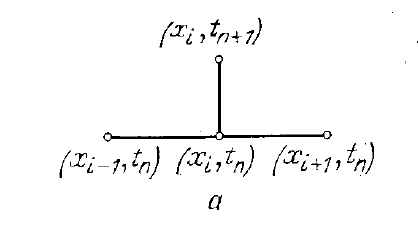
\includegraphics[scale = 0.8]{exp.png} 
\end{center}
\caption{Шаблон для явной схемы}
\end{figure}


Рассмотрим процесс нахождения значений сеточной функции. Сначала заполняем значения на нулевом слое, подставляя значения функции из начального условия $u(x, 0) = \phi(x)$. Далее для слоя с номером $n \in [1; K]$ вычисляем значения внутренних точек по схеме:
$$
\begin{cases}
y_i^n = y_i^{n-1} + \tau\cdot (f_i^{n-1} + \rho(x_i)\cdot y_{x\overline{x}, i}^{n-1}) \\ \\ 
y_{x\overline{x}, i}^{n-1} = \dfrac{y_{i+1}^{n-1} - 2y_i^{n-1} + y_{i-1}^{n-1}}{h^2}
\end{cases}
$$

После этого вычисляем значения в граничных точках, пользуясь граничными условиями:
$$
y_0^n = \dfrac{\mu_1(t^n) + \dfrac{4y_2^n - y_3^n}{2h}}{1 + \dfrac{3}{2h}} ; y_N^n = \dfrac{\mu_2(t^n) + \dfrac{4y_{N-1}^n - y_{N-2}^n}{2h}}{1 + \dfrac{3}{2h}} 
$$
Заметим, что производные в граничных условиях аппроксимируются по трёхточечному шаблону с порядком точности $O(h^2)$:

$$
\bigg( \dfrac{\partial u}{\partial x} \bigg)_0 = \dfrac{-3y_0^n + 4y_1^n - y_3^n}{2h}; 
\bigg( \dfrac{\partial u}{\partial x} \bigg)_N = \dfrac{3y_N^n - 4y_{N-1}^n + y_{N-2}^n}{2h}; 
$$

\newpage

\subsection{Неявная схема}

\begin{figure}[h]
\begin{center}
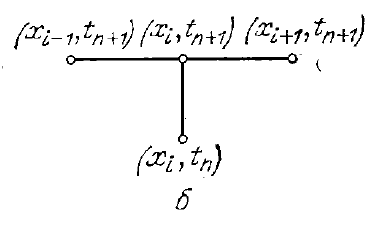
\includegraphics[scale = 0.8]{imp.png} 
\end{center}
\caption{Шаблон для неявной схемы}
\end{figure}

Неявная схема, в отличие от явной, для нахождения значений функции на одном слое требует решения трёхдиагональной системы методом прогонки.
В данной работе был реализован общий вид данной схемы.

Шаблоны по $x$ и по $t$ задаются аналогично, также аналогично первый слой заполняется при помощи начального условия.

Для неявной схемы имеем:

$$
\dfrac{y_i^n - y_i^{n-1}}{\tau} = \rho(x_i) \cdot \bigg(\dfrac{y_{i+1}^n - 2y_i^n + y_{i-1}^n}{h^2} \bigg) + f(x_i, t_n)
$$
Откуда видно, что для каждого слоя будем получать систему уравнений, решение которой ищем методом прогонки.

$$
\begin{cases}
\gamma_i y_{i+1}^n -(1 + 2\gamma_i) y_i^n + \gamma_i y_{i-1}^n = -F_i^n, & i \in {1, N-1} \\ \\
\gamma_i = \dfrac{\tau \cdot \rho(x_i)}{h^2} \\ \\
F_i^n = -y_i^{n-1} + f(x_i, t_n)
\end{cases}
$$

Граничные условия записываются аналогично явной схеме.

$$
\begin{cases}
(\dfrac{3}{2h} + 1)y_0^n - \dfrac{4}{2h}y_1^n + \dfrac{1}{2h}y_2^n = \mu_1(t_n) \\ \\
(\dfrac{3}{2h} + 1)y_N^n - \dfrac{4}{2h}y_{N-1}^n + \dfrac{1}{2h}y_{N-2}^n = \mu_1(t_n)
\end{cases} 
$$

\newpage
\subsection{Симметричная схема}

Рассмотрим разностные выражения, использующиеся в симметричной схеме.

$$
\dfrac{y_i^n - y_i^{n-1}}{\tau} = \dfrac{\rho(x_i)}{2} \cdot \bigg(\dfrac{y_{i+1}^n - 2y_i^n + y_{i-1}^n}{h^2} \bigg) + \dfrac{\rho(x_i)}{2} \cdot \bigg(\dfrac{y_{i+1}^{n-1}- 2y_i^{n-1} + y_{i-1}^{n-1}}{h^2} \bigg) + f(x_i, t_{n-1} + 0.5\tau)
$$

В данном случае, система уравнений приобретает вид:
$$
\begin{cases}
\gamma_i y_{i+1}^n -(1 + 2\gamma_i) y_i^n + \gamma_i y_{i-1}^n = -F_i^n, & i \in {1, N-1} \\ \\
\gamma_i = \dfrac{\tau \cdot \rho(x_i)}{2h^2} \\ \\
F_i^n = y_i^{n-1} + f(x_i, t_{n-1} + 0.5\tau) + \dfrac{\rho(x_i)}{2} \cdot \bigg(\dfrac{y_{i+1}^{n-1}- 2y_i^{n-1} + y_{i-1}^{n-1}}{h^2} \bigg)
\end{cases}
$$

Граничные условия по сравнению с чисто неявной схемой не изменяются.

\begin{figure}[h]
\begin{center}
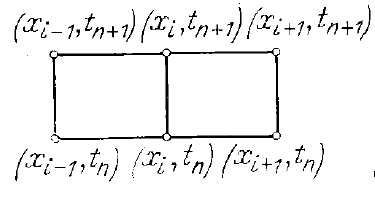
\includegraphics[scale = 0.8]{sym.png} 
\end{center}
\caption{Шаблон для симметричной схемы}
\end{figure}

Можно рассматривать неявные схемы в общем виде, если ввести в разностную схему параметр $\sigma$.

$$
\dfrac{y_i^{n} - y_i^{}}{\tau} = \rho(x) \cdot (\sigma y_{\overline{x}x}^n + (1-\sigma)y_{\overline{x}x}^{n-1}) + f(x_i, t_{n-1}+ \tau \cdot \sigma)
$$

Тогда запишем общий вид матрицы для слоя с номером $n$:

$$
\left(\begin{array}{ccccc|c}
	3+2h & -4 &  1 & 0 & ... & 2h\mu_1(t_n) \\
	\gamma_1 & -1-2\gamma_1 & \gamma_1 & 0 & ... & -F_2^n \\
	0 & \gamma_2 & -1-2\gamma_2 & \gamma_2 & ... & -F_3^n \\
	... & ... & ... & ... & ... &  ... \\
	... & 0 & \gamma_{N-1} & -1-2\gamma{N-1} & \gamma_{N-1} & -F_{N-1}^n \\
	... & 0 & 1 & -4 & 3+2h & 2h\mu_2(t_n) 
\end{array}\right)
$$
Где:
$$
\gamma_i = \dfrac{\tau \rho(x_i) \sigma}{h^2}, i \in \overline{1, N-1}
$$

Эта система строится для каждого слоя, затем приводится к трёхдиагональному виду и решается методом прогонки. 
Также в выражениях для коэффициентов фигурирует $\sigma$. Для чисто неявной схемы считаем $\sigma=1$. Полагая $\sigma=\dfrac{1}{2}$, получаем симметричную схему. Если взять $\sigma = 0$, получим явную схему.

\section{Результаты}
\subsection{Явная схема}
\begin{enumerate}
\item Определение числа разбиений для достижения заданной точности \\
Требуемая точность $\varepsilon_0 = 10^{-3}$

Достаточно просто определить, что для $M_1 = 120000$ и $M_2 = 150000$ выполняется неравенство: $\varepsilon(M_2) < \varepsilon_0 < \varepsilon(M_1)$

Для того, чтобы найти $M_0: \varepsilon(M_0) < \varepsilon_0 < \varepsilon(M_0 - 1)$, воспользуемся методом половинного деления интервала $[M_1;M_2]$.Ниже приведена таблица значений, близких к искомому $M_0$

\begin{table}[H]
\caption{Зависимость погрешности от числа разбиений по $x$ }
\begin{center}
\begin{tabular}{|c|c|}
\hline
$N$ & $\varepsilon_N$ \\
\hline
136962 & 1.000309e-03 \\
\hline
136977 & 1.000090-03  \\
\hline
136980 & 1.000046e-03 \\
\hline
136982 & 1.000017e-03 \\
\hline
136983 & 1.000002e-03 \\
\hline
$M_0 = 136984$ & 9.999876e-04 \\
\hline
\end{tabular}
\end{center}
\end{table}

Где $\varepsilon$ вычисляется по формуле

$$
\varepsilon = \dfrac{||u -v||_{h\tau}}{||u||_{h\tau}},  ||u||_{h\tau} = \max \limits_{{t\in[0,T]}}||u(t)||_h
$$
В качестве нормы по $h$ используется бесконечная норма $||u(t)||_h = \max \limits_{{i\in[0,N]}}(u(x_i, t))$, 
для которой будет выполнено условие согласованности норм для нашей задачи.

\newpage

\item Графики зависимостей значений сеточной функции от $x$ и $t$ при различных последовательных значениях $t$.

\begin{figure}[H]
\centerline{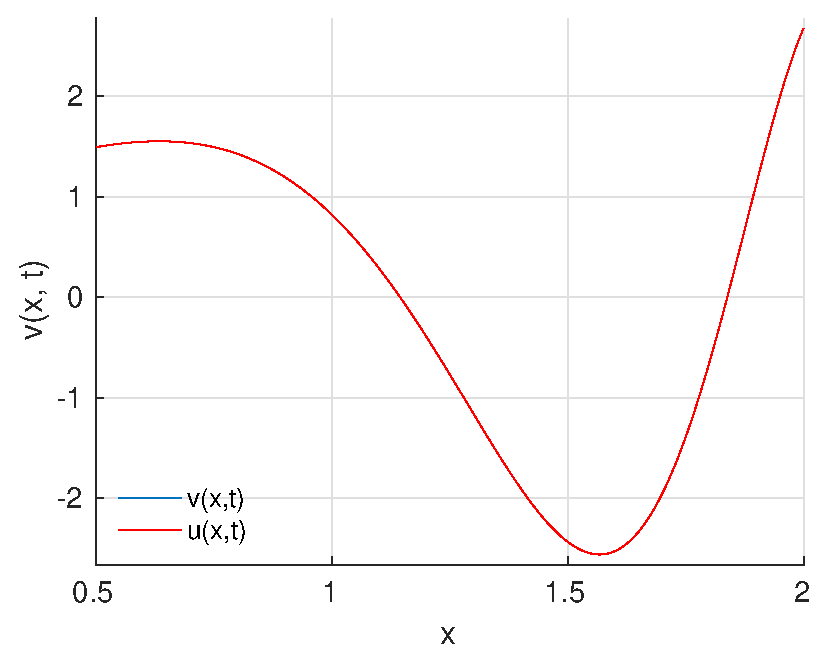
\includegraphics[scale = 0.7]{exp_t=1.eps}}
\caption{Явная схема, $h_0 = \dfrac{1.5}{M_0}, \tau_0 = \dfrac{h^2}{2 \cdot q(2)}, t = 0$}
\end{figure} 

\begin{figure}[H]
\centerline{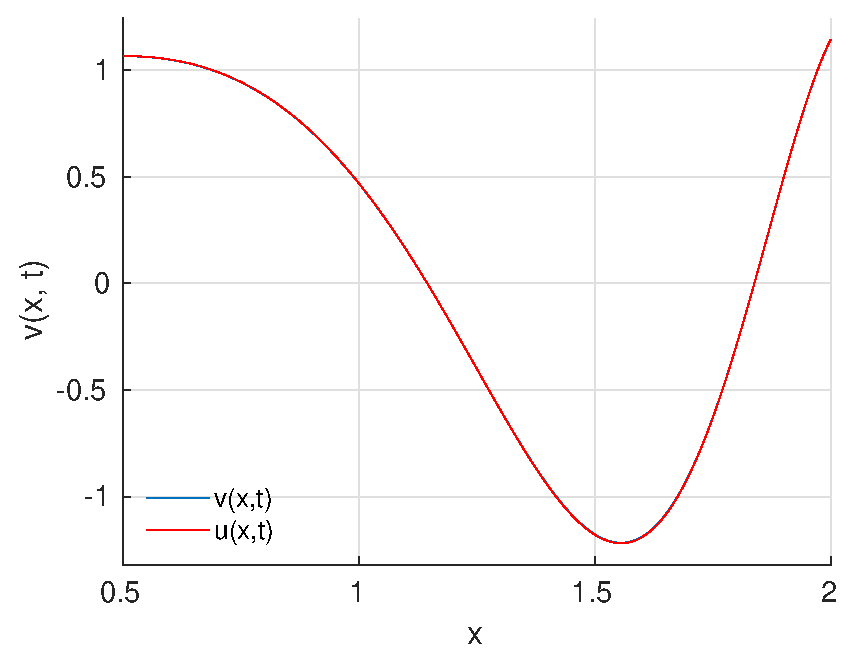
\includegraphics[scale = 0.7]{exp_t=655.eps}}
\caption{Явная схема, $h_0 = \dfrac{1.5}{M_0}, \tau_0 = \dfrac{h^2}{2 \cdot q(2)}, t = 655$}
\end{figure} 

\begin{figure}[H]
\centerline{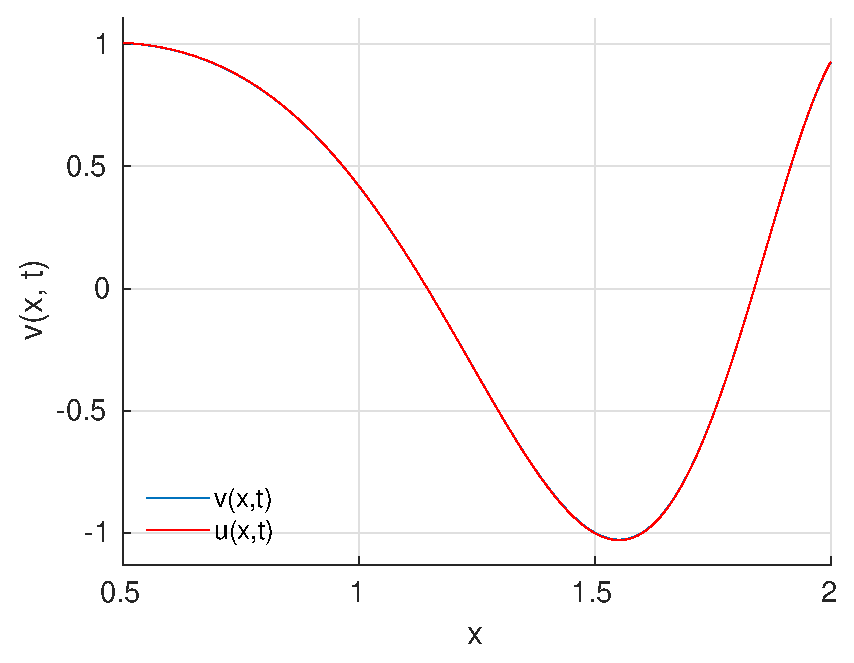
\includegraphics[scale = 0.7]{exp_t=1309.eps}}
\caption{Явная схема, $h_0 = \dfrac{1.5}{M_0}, \tau_0 = \dfrac{h^2}{2 \cdot q(2)}, t = 1309$}
\end{figure} 

\begin{figure}[H]
\centerline{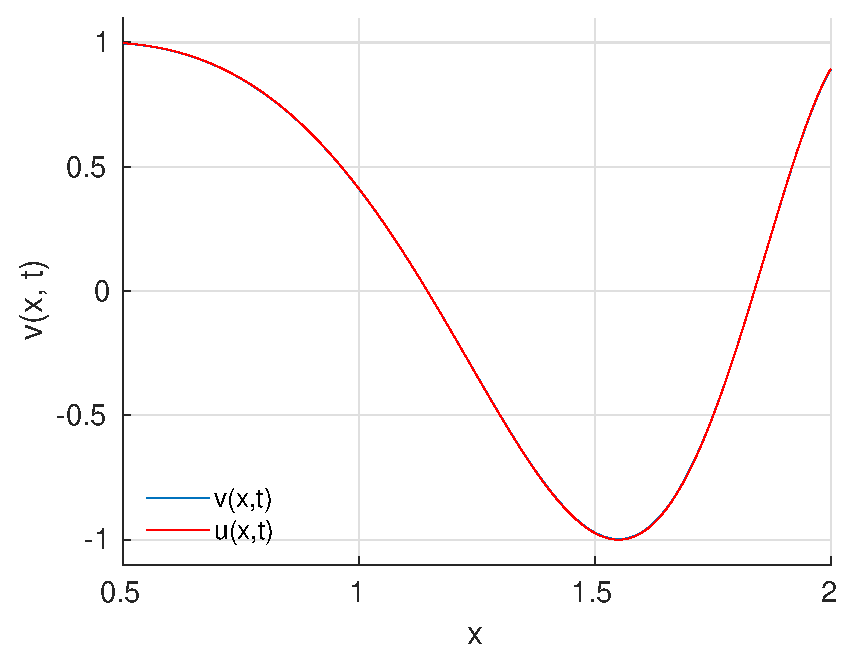
\includegraphics[scale = 0.7]{exp_t=2617.eps}}
\caption{Явная схема, $h_0 = \dfrac{1.5}{M_0}, \tau_0 = \dfrac{h^2}{2 \cdot q(2)}, t = 2617$}
\end{figure} 

\item{Иллюстрация неустойчивости}

Возьмём $\tau = \tau_0 + \delta, \delta = 1.85e-5$ и число разбиений по $x$ $N = 10000$. Построим аналогичные графики сечений, только теперь сечения по оси $x$. Неустойчивость явно проявляется ближе к правой границе по $x$, соответственно будем рассматривать сечения в окрестности этой границы.

\begin{figure}[H]
\centerline{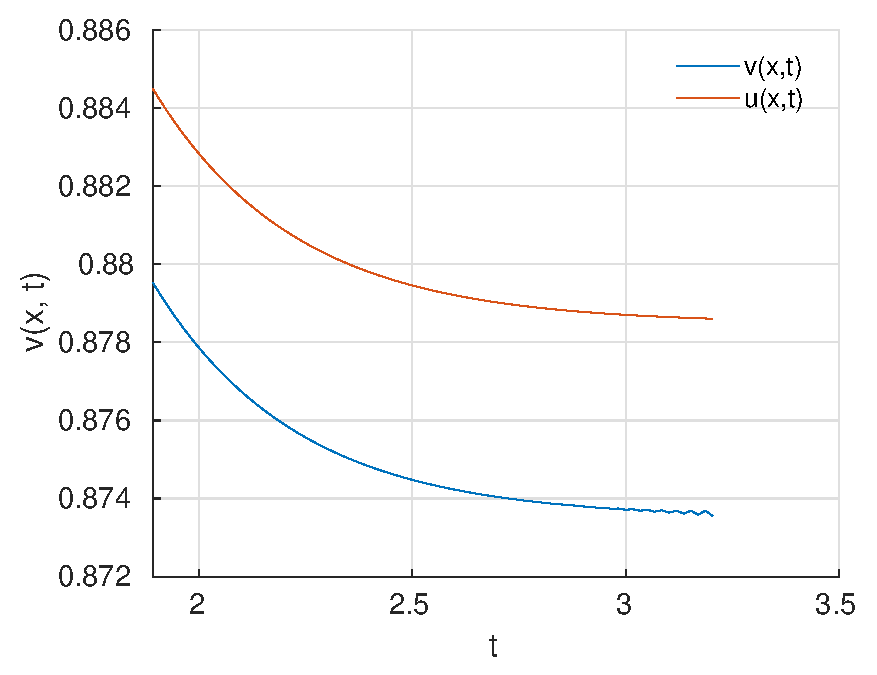
\includegraphics[scale = 0.7]{instable_x=1995.eps}}
\caption{Явная схема, неустойчивость,$h_0 = \dfrac{1.5}{M_0}, \tau, x_{ind} = 1995$}
\end{figure} 

\begin{figure}[H]
\centerline{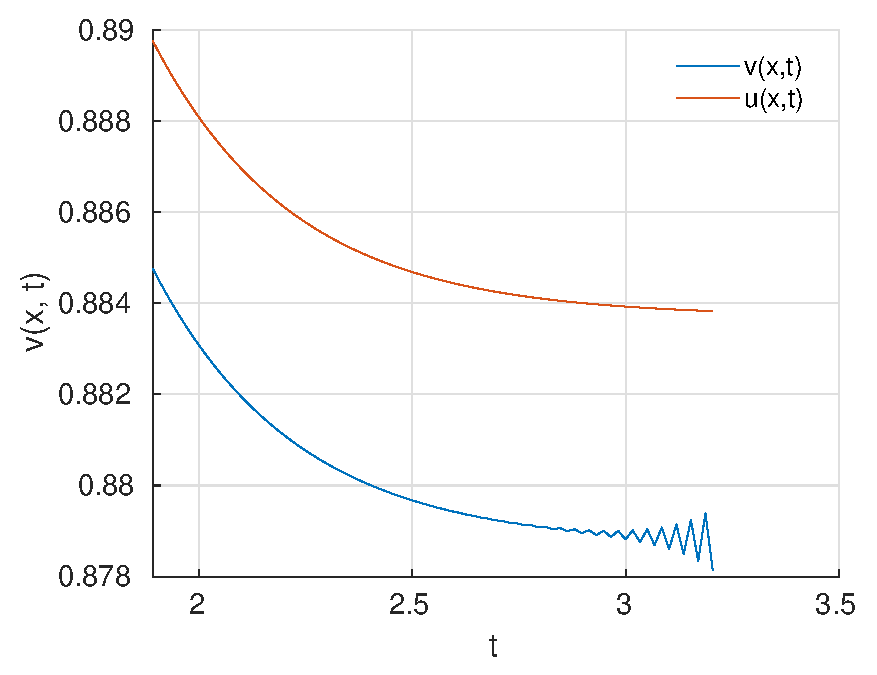
\includegraphics[scale = 0.7]{instable_x=1997.eps}}
\caption{Явная схема, неустойчивость,$h_0 = \dfrac{1.5}{M_0}, \tau, x_{ind} = 1997$}
\end{figure} 

\begin{figure}[H]
\centerline{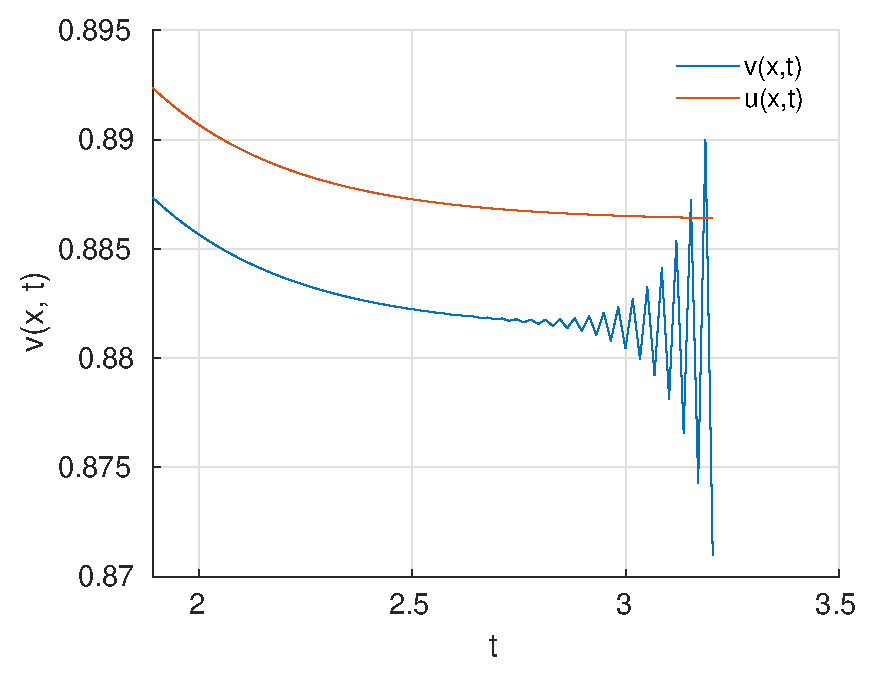
\includegraphics[scale = 0.7]{instable_x=1998.eps}}
\caption{Явная схема, неустойчивость,$h_0 = \dfrac{1.5}{M_0}, \tau, x_{ind} = 1998$}
\end{figure} 

\begin{figure}[H]
\centerline{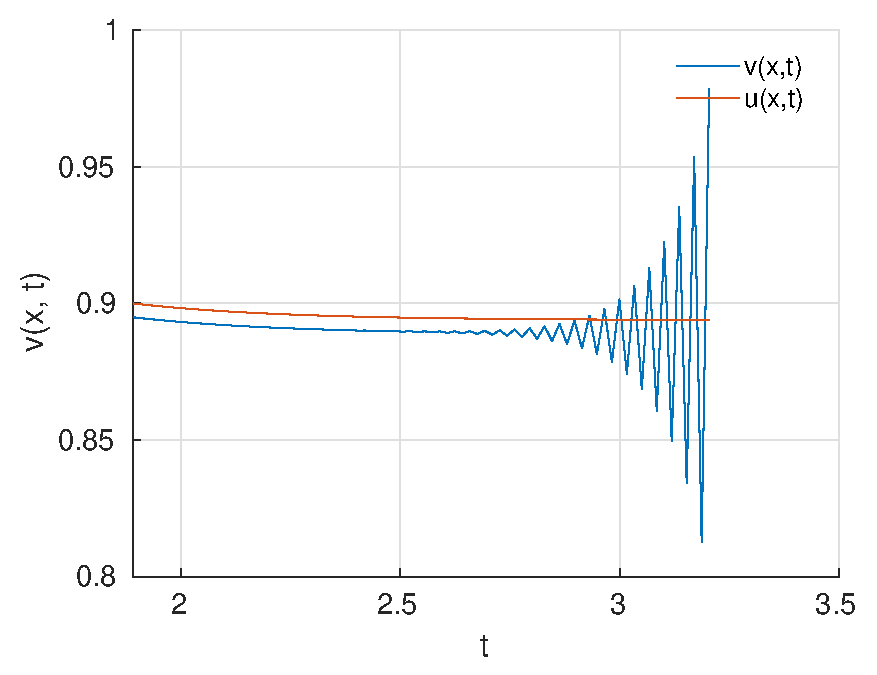
\includegraphics[scale = 0.7]{instable_x=2001.eps}}
\caption{Явная схема, неустойчивость,$h_0 = \dfrac{1.5}{M_0}, \tau, x_{ind} = 2001$}
\end{figure} 

По графикам легко заметить, что функции перестали совпадать совершенно. Даже при малейшем  увеличении максимально доступного из условия устойчивости $\tau$, ошибка возрастает колоссально. Для данного конкретного $\tau: \varepsilon_{\tau} = 1.452027e+220$
 
\end{enumerate}

\newpage

\subsection{Неявная схема}
Исследуем, на сколько можно увеличить шаг по времени начиная от $\tau_0$, сохранив при этом требуемую точность.

\begin{figure}[H]
\centerline{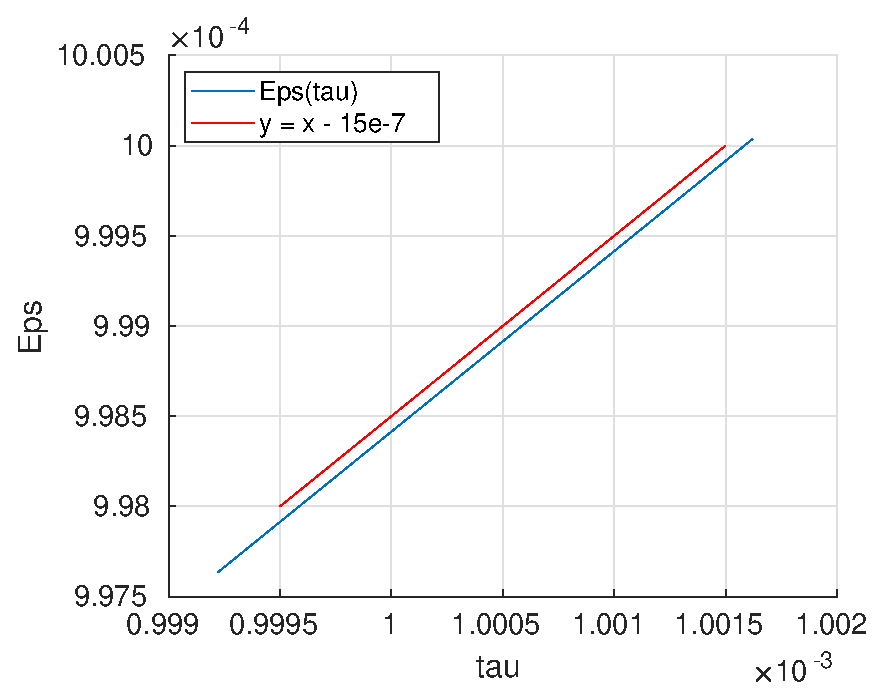
\includegraphics[scale = 0.7]{epstau.eps}}
\caption{Неявная схема, $\varepsilon(\tau)$}
\end{figure} 


\subsection{Симметричная схема}
Проведём исследование, аналогичное тому, что было в неявной схеме.

\begin{figure}[H]
\centerline{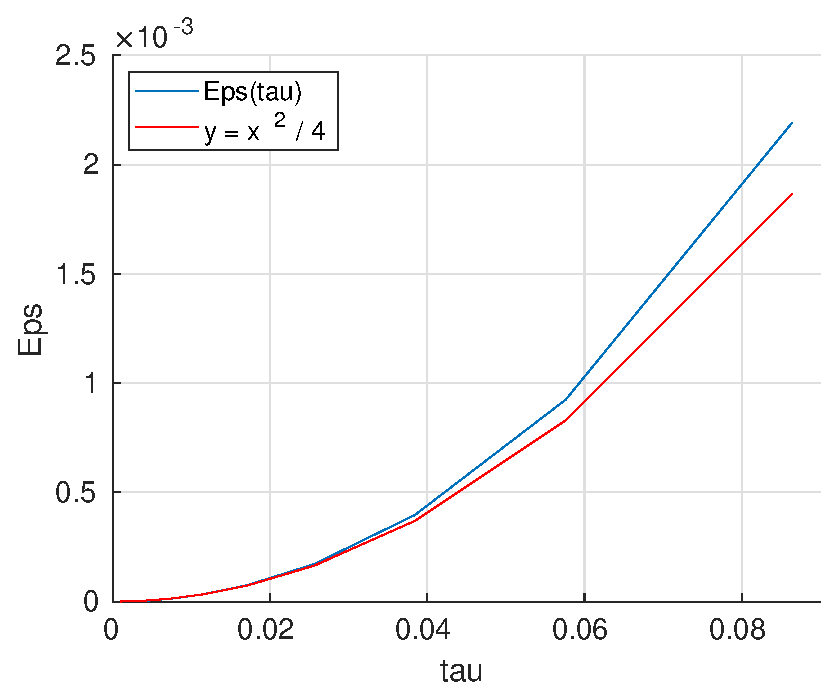
\includegraphics[scale = 0.7]{epstausym.eps}}
\caption{Симметричная схема, $\varepsilon(\tau)$}
\end{figure} 


\subsection{Сравнение схем}
Произведём сравнение трёх схем. Будем сравнивать схемы по времени работы при одном и том же числе разбиений по $h$ и по $t$, а также проверим порядок аппроксимации для каждой схемы.

Ниже приведена сводная таблица с исследованиями. (рассматриваем фиксированный шаг $h$, считаем $\tau = \dfrac{h^2}{2q(2)}$ при всех замерах). 

\begin{table}[H]
\caption{Таблица для проверки порядков аппроксимации разностных схем}
\begin{center}
\begin{tabular}{|c|c|c|c|c|}
\hline
$h$ & $tau$ & $\varepsilon$, Явная схема & $\varepsilon$, Неявная схема & $\varepsilon$, Симметричная схема  \\
\hline
6e-4 & 3 & 1.426942e+1 & 1.779575 & 1.604145 \\
\hline
3e-4 & 7.5 & 2.321806 & 1.126013 & 2.811328e-1  \\
\hline
1.5e-4 & 0.1875 & 2.867224e-1 & 2.377931e-1 & 1.217982e-2 \\
\hline
7.5e-5 & 4.6875e-2 & 5.244476e-2 & 5.004149e-2 & 5.994168e-4 \\ 
\hline
3.75e-5 & 1.171875e-2 & 1.203692e-2 & 1.189528e-2 & 3.436387e-5 \\
\hline
1.875e-5 & 2.929687e-3 & 2.944778e-3 & 2.934803e-3 & 1.653247e-6 \\
\hline
9.375e-6 & 7.324219e-4 & 7.326762e-4 & 7.307866e-4 & 5.428163e-7 \\
\hline
\end{tabular}
\end{center}
\end{table}

\begin{table}[H]
\caption{Оценка трудоёмкости разностных схем по времени работы}
\begin{center}
\begin{tabular}{|c|c|c|c|}
\hline
$\varepsilon$ & $t$, Явная схема & $t$, Неявная схема & $t$, Симметричная схема  \\
\hline
0.1 & 0.08 & 0.16 & 0.02 \\
\hline
0.01 & 0.6 & 0.87 & 0.13\\
\hline
0.001 & 185 & 55 & 0.67\\
\hline
\end{tabular}
\end{center}
\end{table}

Время в таблице указано в секундах.

\section{Выводы}
В результате сравнения трёх схем можно сделать определённые выводы. С ростом числа разбиений симметричная схема в десятки раз эффективнее по скорости работы, нежели явная или даже чисто неявная схема, всвязи с чем ей стоит отдавать предпочтение при реальных расчётах.

\section{Приложения}
Исходные файлы лабораторной работы можно найти тут: \\
\url{https://github.com/LanskovNV/numerical-analysis/tree/master/%D0%A1%D0%B5%D1%82%D0%BE%D1%87%D0%BD%D1%8B%D0%B5%20%D0%BC%D0%B5%D1%82%D0%BE%D0%B4%D1%8B/lab_2}
\end{document}

